\chapter{API-integráció és kliensoldali biztonság}

A WaccApp frontendjének működésében az API-integráció nem önálló technikai háttérrészlet, hanem a felhasználói műveletek közvetlen folytatása. A korábbi fejezetek bemutatták, hogy a rendszer több, feladat szerint elkülönített nézetből áll, és ezek a nézetek különböző kommunikációs, kérdőíves, szűrési, média- és időzítési folyamatokat támogatnak. Ebben a fejezetben az kerül bemutatásra, hogy a WaccApp egyes frontendműveletei milyen szerveroldali végpontokhoz kapcsolódnak, és a kliensoldal hogyan kezeli az ezekből érkező válaszokat. 

A frontend szempontjából az API-kapcsolat minden esetben egy felhasználói döntésből indul. A felhasználó üzenetet küld, sablont választ, kérdőívet indít, fájlt csatol, szűrést futtat, beszélgetést nyit meg vagy időzített műveletet állít be. A kliensoldal ezekből az adatokból állítja össze azt a kérést, amelyet a háttérrendszer felé továbbít. A válasz megérkezése után a frontend feladata az, hogy a technikai eredményt felhasználói szempontból értelmezhető állapottá alakítsa. Ez lehet sikeres küldés, hiányzó adat miatti hiba, üres találati lista, sikertelen fájlküldés, nem létező kérdőív, vagy egy időzített művelet mentésének eredménye. 

A fejezet másik fontos célja a kliensoldali felelősség határainak tisztázása. Ez különösen fontos azért, mert a WaccApp nemcsak technikai kéréseket továbbít, hanem telefonszámokkal, üzenetekkel, kérdőíves válaszokkal és médiatartalmakkal dolgozó kommunikációs felületként működik. A WaccApp frontendje nem helyettesíti a backendoldali ellenőrzést, a jogosultságkezelést vagy a WhatsApp Business Platform szabályainak érvényesítését. Ugyanakkor első védelmi és értelmezési rétegként működik: csökkenti a hibás kérések számát, segíti a helyes adatbevitelt, óvatosan kezeli a megjelenített adatokat, és a felhasználó számára láthatóvá teszi azokat a korlátozásokat, amelyek a platform- vagy adatvédelmi működésből következnek. [R10], [R11], [R12]

Az API-integráció megértéséhez érdemes a WaccApp működését rendszerarchitektúra szintjén is áttekinteni. A \ref{fig:rendszer-architektura}. ábra azt mutatja meg, hogy a felhasználói művelet hogyan halad végig a frontendrétegen, a REST API-kapcsolaton, a backend feldolgozáson, a WhatsApp Business API-integráción és az adatbázison.

\begin{figure}[H]
\centering
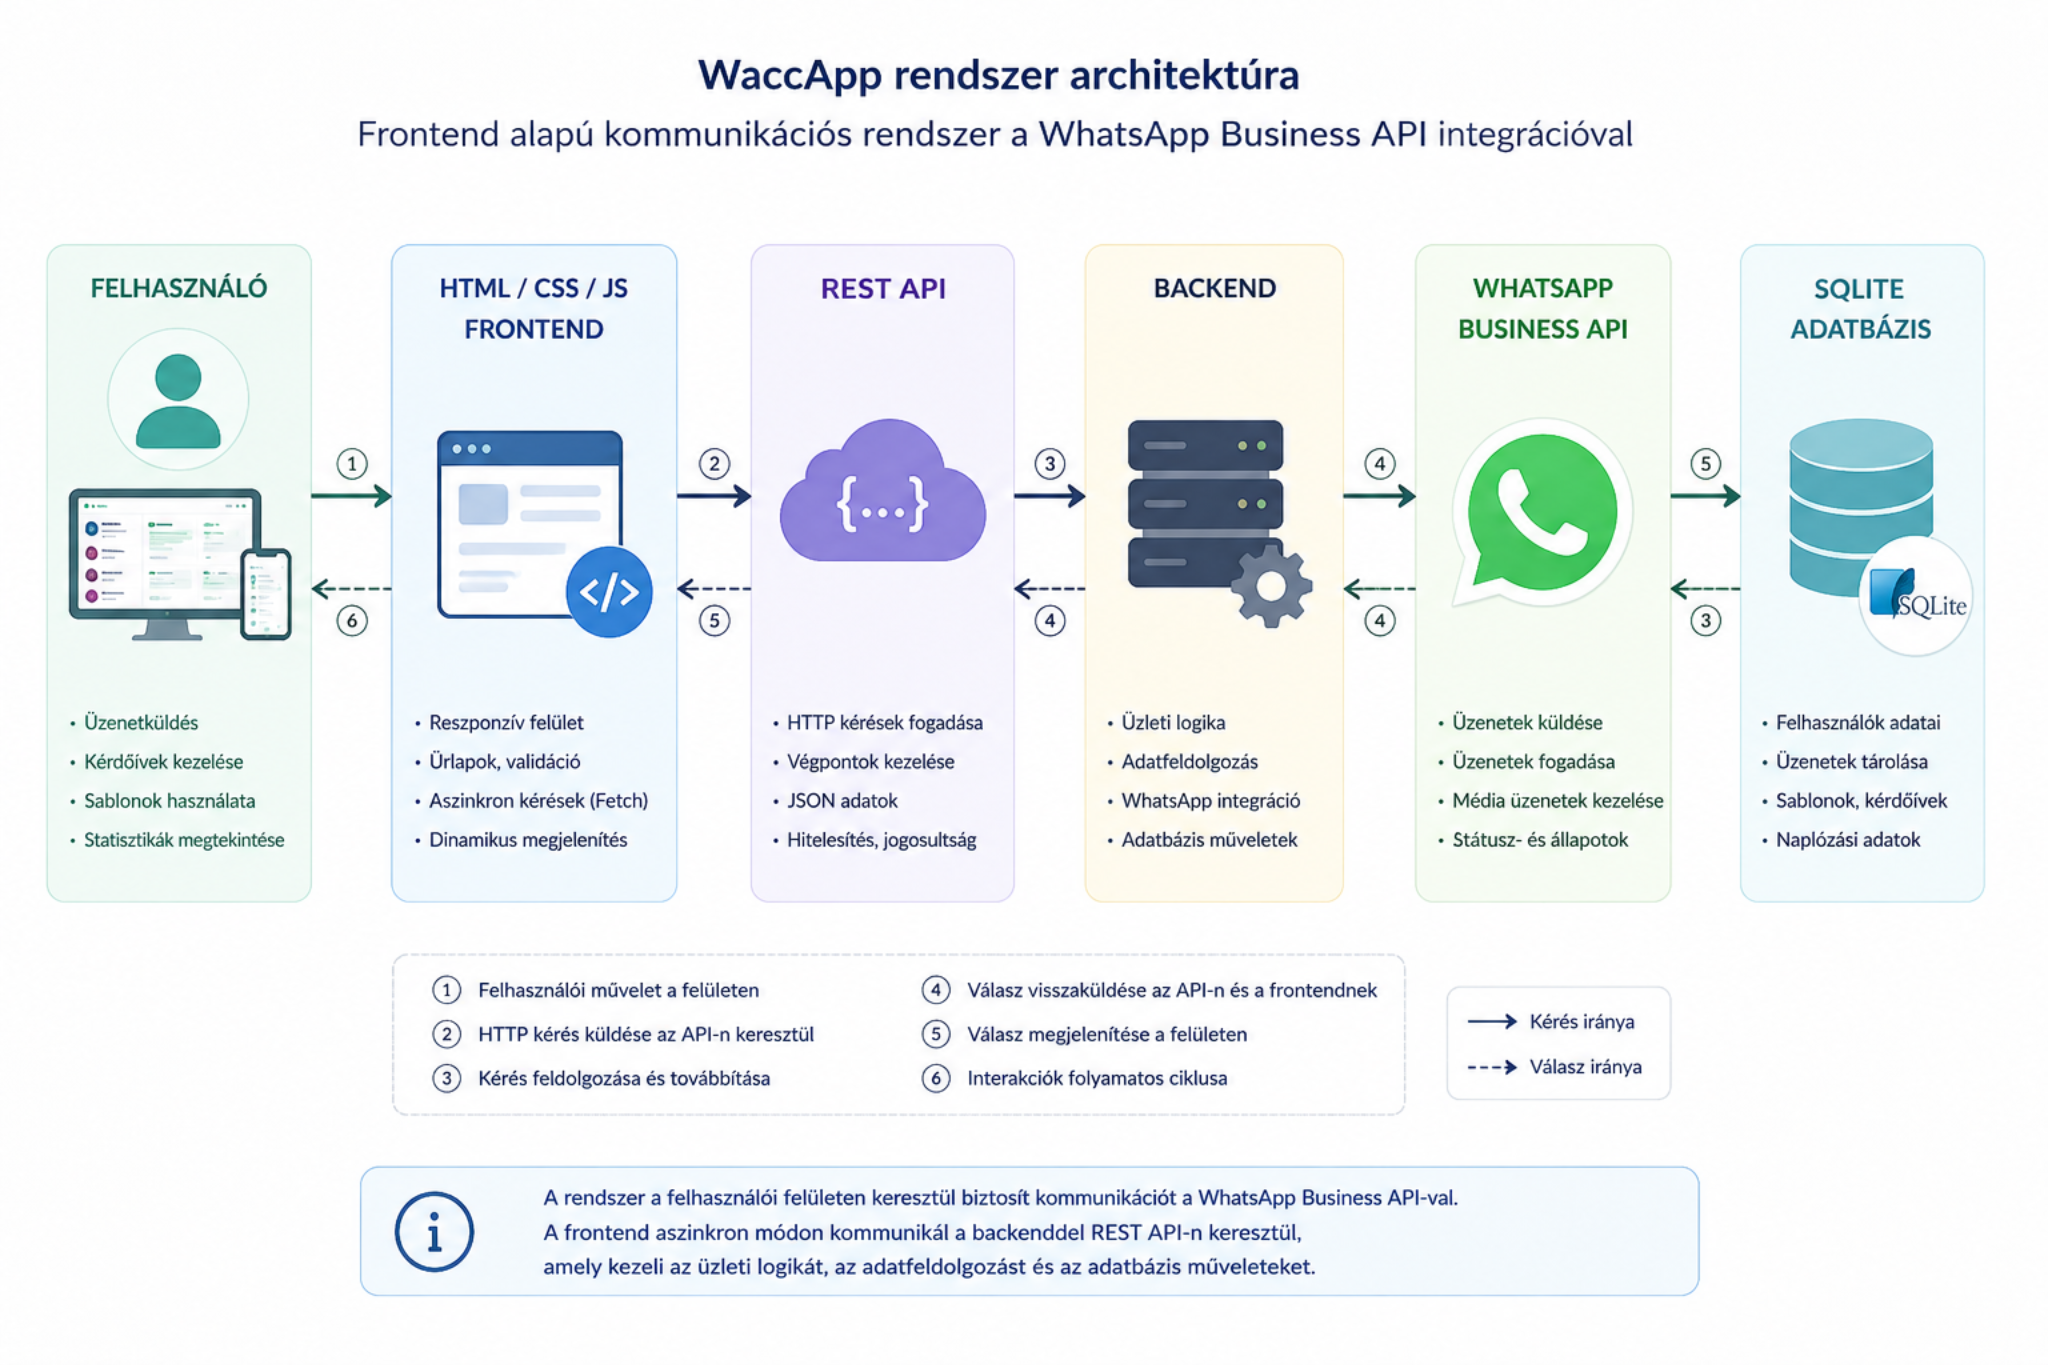
\includegraphics[width=0.95\textwidth]{images/waccapp-rendszer-architektura.png}
\caption{A WaccApp rendszer architektúrája frontend nézőpontból.}
\label{fig:rendszer-architektura}
\end{figure}

A frontend a felhasználói műveletek kiindulópontja és a visszajelzések megjelenítési helye, de a tényleges üzenetküldés, adattárolás és WhatsApp-platformmal való kommunikáció a háttérrendszeren keresztül történik. Ezért a WaccApp kliensoldala köztes értelmező rétegként működik: a felhasználó számára kezelhető űrlapokat, nézeteket és állapotokat ad, miközben a háttérben REST API-kérések kapcsolják össze a felületet a szerveroldali logikával és a külső kommunikációs platformmal.

\section{Az API-kapcsolatok szerepe a frontend moduljaiban}

A WaccApp frontendnézetei eltérő típusú API-kapcsolatokat használnak. Az \path{index.html} elsősorban műveletindító oldal, ezért innen főként olyan kérések indulnak, amelyek valamilyen kommunikációs műveletet hajtanak végre. Ide tartozik az egyedi szöveges üzenet küldése, a sablonos üzenet továbbítása, a fájl- vagy médiaküldés, a kérdőív indítása, valamint az időzített küldések rögzítése. Ebben a nézetben a frontend szerepe az, hogy a felhasználó által kiválasztott küldési módhoz igazítsa az adatokat, majd a megfelelő végpont felé továbbítsa a kérést. 

A kommunikációs előzményekhez kapcsolódó nézetek más jellegű API-kapcsolatokat igényelnek. A \path{messages.html}, a \path{sent-messages.html} és a \path{conv.html} nem elsősorban új műveleteket hoznak létre, hanem meglévő kommunikációs adatokat kérnek le és jelenítenek meg. A frontend itt a szerveroldalról érkező üzenetadatokat alakítja át listává, beszélgetésfolyammá vagy kontaktalapú nézetté. A \path{conv.html} esetében különösen fontos, hogy a beérkező adatok időrendi és típus szerinti értelmezést kapjanak, mert a felhasználó nem technikai rekordokat, hanem beszélgetést szeretne látni. 

A kérdőív- és sablonkezelő oldalak szintén saját API-kapcsolati logikával rendelkeznek. A \path{questionnaire.html} és a \path{template.html} esetében a frontend nemcsak adatokat kér le, hanem szerkesztett struktúrákat is ment. A kérdések, válaszok, elágazások, sablonnevek és gombos kapcsolatok olyan szerkezetet alkotnak, amelyet a háttérrendszernek később kérdőívindításkor vagy sablonos kommunikáció során újra fel kell tudnia használni. Emiatt ezeknél a nézeteknél az API-integráció nem egyszerű adatlekérdezés, hanem a szerkesztett kommunikációs logika tárolásának és visszatöltésének eszköze. 

A \path{filter.html} API-kapcsolatai visszakeresési és értelmezési célt szolgálnak. Ez az oldal a korábbi kommunikációs események, kérdőívválaszok és metaadatok alapján állít elő szűrt eredményeket. A frontend itt a felhasználó által megadott feltételeket, például nevet, telefonszámot, dátumintervallumot, üzenettípust vagy kérdőívhez kapcsolódó adatot alakít lekérdezhető formává. Az API-válasz alapján a felület nem pusztán adatokat ír ki, hanem áttekinthető eredménymegjelenítést biztosít. 

A belépési, adminisztratív és fiókkezelő oldalak más jellegű kapcsolatot képviselnek. A \path{login.html}, az \path{account.html} és az \path{admin.html} esetében a frontend olyan végpontokhoz kapcsolódik, amelyek a hozzáféréshez, fiókadatokhoz, adminisztratív beállításokhoz vagy hozzájárulások kezeléséhez tartoznak. Ezek a nézetek nem a kommunikációs folyamat közvetlen magját adják, de fontosak abból a szempontból, hogy a rendszer használata ellenőrzött keretek között történjen. 

\section{A frontend szempontból fontos végpontok működési csoportjai}

A WaccApp-ban az üzenetküldési folyamatokhoz több, egymástól eltérő célú végpont kapcsolódik. Az egyedi szöveges üzenetek küldését a /send-message végpont szolgálja, amelyhez a frontend jellemzően a címzettet és az üzenettartalmat továbbítja. A sablonos üzenetek esetében a /send-template végpont kap szerepet, ahol a kliensoldalnak már nemcsak címzettet, hanem sablonnevet, nyelvi beállítást és adott esetben paramétereket is kezelnie kell. A fájl- és médiaküldéshez a /send-file-message kapcsolódik, amelynél a frontendnek a szöveges adatok mellett a kiválasztott állományt is továbbítania kell. Ezek a végpontok ugyan mind küldési művelethez tartoznak, de eltérő adatbeviteli helyzetet eredményeznek, ezért az \path{index.html} felületén a mezők és ellenőrzések a választott küldési típushoz igazodnak. 

A kérdőíves és sablonos működéshez lekérdező és mentő végpontok is kapcsolódnak. Az /available-templates, az /available-template-questionnaires és a /firsttemplates a választható sablonok, sablonos kérdőívek és kezdősablonok betöltését támogatják. A /get-questionnaire/:theme és az /all-questionnaires a kérdőívek betöltéséhez és áttekintéséhez kapcsolódik. A szerkesztési oldalon a /save-to-questionnaire a kérdőíves logika mentésében kap szerepet, míg a /create-template a sablonkészítéshez kötődik. A frontend számára ezek a végpontok azért különösen fontosak, mert a kérdőívszerkesztés nem statikus űrlapkitöltés, hanem a háttérrendszerből érkező és oda visszamentett folyamatstruktúrákra épül. 

A kommunikációs előzmények és visszakereshető adatok megjelenítését elsősorban a /messages, a /sent-messages, a /contacts, a /message-metadata és a /questionnaire-themes végpontok támogatják. A /messages a beérkező vagy tárolt kommunikációs események lekéréséhez kapcsolódik, míg a /sent-messages az elküldött tételek megjelenítését segíti. A /contacts a kontaktalapú működésben fontos, mert a beszélgetésnézet és a szűrés is támaszkodhat a név és telefonszám közötti kapcsolatra. A /message-metadata és a /questionnaire-themes olyan kiegészítő adatokat biztosítanak, amelyek a szűrési és értelmezési folyamatokat támogatják. Ezek a végpontok elsősorban a \path{messages.html}, a \path{sent-messages.html}, a \path{conv.html} és a \path{filter.html} működéséhez kapcsolódnak. 

Az időzített műveletekhez a /schedule és a /schedule-media végpontok tartoznak. A /schedule az időzített szöveges, sablonos vagy kérdőíves műveletek rögzítéséhez használható, míg a /schedule-media a médiatartalomhoz kapcsolódó ütemezést támogatja. Frontendoldalon ezek a végpontok azért igényelnek külön figyelmet, mert az időzítésnél a művelet rögzítése és tényleges végrehajtása időben elválik egymástól. Az \path{index.html} ezért nemcsak azt kezeli, hogy mit szeretne küldeni a felhasználó, hanem azt is, hogy mikor történjen meg a küldés. 

Az adminisztratív és hozzáférési funkciókhoz olyan végpontok kapcsolódnak, mint az /admin/auth/login, az /admin/me, az /admin/account, az /admin/users, az /admin/consents és az ezekhez tartozó módosító vagy törlő végpontok. Ezek szerepe frontend szempontból az, hogy a belépési, fiókkezelési és adminisztratív nézetek ne közvetlenül a háttérrendszer belső működését érjék el, hanem szabályozott API-kapcsolatokon keresztül dolgozzanak. A \path{login.html}, az \path{account.html} és az \path{admin.html} így a kommunikációs moduloktól eltérő, de a rendszer egészéhez szükséges kapcsolódási réteget képviselnek.  A frontend szempontból fontosabb végpontok összefoglaló táblázata a 15.2. mellékletben található.

\section{Konkrét API-hívási példák frontend nézőpontból}

A végpontok működési csoportjai mellett érdemes néhány konkrét API-hívási példán keresztül is bemutatni, hogyan kapcsolódik a WaccApp frontendje a háttérrendszerhez. Ezek a példák azt mutatják meg, hogy a kliensoldal milyen adatot állít össze, milyen végpontra küldi azt, és a kapott válasz alapján hogyan módosítja a felület állapotát. Frontend szempontból tehát nem önmagában az API-végpont a fő kérdés, hanem az, hogy a felhasználói művelet hogyan alakul át HTTP-kéréssé, majd felhasználói visszajelzéssé.

Az egyik legegyszerűbb és legjobban értelmezhető példa az egyedi szöveges üzenet küldése. Ebben az esetben az \path{index.html} felületén a felhasználó megadja a címzett telefonszámát és az üzenet szövegét. A frontend a küldés előtt ellenőrzi, hogy a szükséges mezők ki vannak-e töltve, majd JSON-formátumban továbbítja az adatokat a /send-message végpontra.

\begin{CodeBlock}
POST /send-message
Content-Type: application/json
{
  "phone": "+36301234567",
  "message": "Szia! Ez egy teszt üzenet.",
  "content": "Szia! Ez egy teszt üzenet.",
  "theme": null
}
\end{CodeBlock}

A kérésben a phone mező jelöli a címzettet, a message mező tartalmazza a ténylegesen elküldendő szöveget, a content mező pedig a későbbi naplózás vagy kérdőíves folyamatok miatt használható kiegészítő tartalomként. Egyszerű üzenetküldésnél a message és a content értéke azonos is lehet. A theme mező opcionális, és akkor kap szerepet, ha az üzenet kérdőíves vagy tematikus kommunikációs folyamathoz kapcsolódik.

A backend válasza sikeres küldés esetén nem pusztán egy technikai státuszkód, hanem olyan JSON-válasz, amelyből a frontend eldöntheti, hogy milyen visszajelzést kell megjelenítenie a felhasználónak. Egy egyszerűsített válasz például a következő formában értelmezhető:

\begin{CodeBlock}
{
  "message": "Az üzenetküldés sikeresen lezárult",
  "results": [
    {
      "phone": "+36301234567",
      "status": "success",
      "response": {
        "messages": [
          {
            "id": "wamid.pelda_uzenetazonosito"
          }
        ]
      }
    }
  ]
}
\end{CodeBlock}

A frontend ebből elsősorban nem a WhatsApp által visszaadott belső azonosítót jeleníti meg, hanem a művelet eredményét értelmezi. Ha a results tömbben az adott címzetthez success állapot tartozik, akkor a felület sikeres küldési visszajelzést adhat. Ha ugyanebben a szerkezetben error állapot jelenik meg, akkor a frontend hibás műveletként kezeli a választ, és olyan üzenetet jelenít meg, amelyből a felhasználó érti, hogy a küldés nem zárult sikeresen.

A második példa a kommunikációs előzmények lekéréséhez kapcsolódik. A messages.html, a \path{conv.html} és részben a \path{filter.html} működéséhez szükség van a korábban beérkezett üzenetek lekérésére. Ezt a frontend a /messages végpont meghívásával éri el.

\begin{CodeBlock}
GET /messages
\end{CodeBlock}

A válasz egy üzenetrekordokat tartalmazó JSON-tömb. Egy egyszerűsített válaszrészlet például így nézhet ki:

\begin{CodeBlock}
[
  {
    "ID": 12,
    "Phone\_number": "+36301234567",
    "Name": "Teszt Elek",
    "Body": "Igen",
    "Type": "button",
    "Received\_at": "2026-05-07 10:42:15"
  },
  {
    "ID": 11,
    "Phone\_number": "+36301234567",
    "Name": "Teszt Elek",
    "Body": "Szia!",
    "Type": "text",
    "Received\_at": "2026-05-07 10:40:02"
  }
]
\end{CodeBlock}

Ebben az esetben a frontend feladata nem merül ki abban, hogy a kapott adatokat változtatás nélkül kiírja a képernyőre. A \path{messages.html} listaalapú formában jeleníti meg az üzeneteket, a \path{conv.html} pedig ugyanilyen jellegű adatokból beszélgetésfolyamot épít. A kliensoldal a Phone\_number, Name, Body, Type és Received\_at mezők alapján dönti el, hogy melyik kontakthoz tartozik az üzenet, milyen tartalom jelenjen meg, milyen típusú üzenetről van szó, és az időrendben hol kell elhelyezni azt. A felhasználó így nem adatbázisrekordokat lát, hanem értelmezhető kommunikációs előzményt.

Hasonló logikát használ az elküldött üzenetek lekérése is. A /sent-messages végpont azokat a tartalmakat adja vissza, amelyeket a rendszer korábban elküldött. Ez különösen a \path{sent-messages.html}, a \path{conv.html} és a \path{filter.html} szempontjából fontos.

\begin{CodeBlock}
GET /sent-messages
[
  {
    "id": 25,
    "phone": "+36301234567",
    "type": "text",
    "content": "Szia! Ez egy teszt üzenet.",
    "timestamp": "2026-05-07 10:39:51",
    "media\_url": null,
    "wa_message\_id": "wamid.pelda_uzenetazonosito",
    "theme": null
  }
]
\end{CodeBlock}

A beérkező és elküldött üzenetek szerkezete nem teljesen azonos, ezért a frontendnek ezeket egységes megjelenítési formára kell alakítania. A \path{conv.html} például a beérkező üzeneteket és az elküldött üzeneteket közös időrendi beszélgetésként jeleníti meg. Ehhez a kliensoldalnak irányt kell rendelnie az üzenetekhez, vagyis meg kell különböztetnie, hogy received vagy sent típusú kommunikációs eseményről van szó. Ez a frontend szempontjából fontos átalakítás, mert a felhasználó egy összefüggő beszélgetést akar látni.

A harmadik példa a \path{filter.html} működéséhez kapcsolódik. Ennél a modulnál fontos pontosítani, hogy a WaccApp jelenlegi formájában nem egyetlen külön szűrési végpontot használ minden feltétel kiszolgálására. A \path{filter.html} több meglévő végpontról tölti be az adatokat, majd a szűrési feltételek jelentős részét kliensoldalon alkalmazza. Ez a megoldás a jelenlegi rendszer méretéhez illeszkedik, mert a szűrőfelületnek elsősorban a meglévő üzenet- és kérdőíves adatok áttekinthető visszakeresését kell támogatnia.

A \path{filter.html} működéséhez például a következő lekérések kapcsolódhatnak:

\begin{CodeBlock}
GET /messages
GET /sent-messages
GET /available-templates
GET /questionnaire-themes
GET /get-questionnaire/ugyfel_elegedettseg
\end{CodeBlock}

A /questionnaire-themes végpont a kérdőíves témák listáját adja vissza, a /get-questionnaire/:theme pedig egy kiválasztott kérdőív kérdéseit és válaszlogikáját tölti be. Egy egyszerűsített kérdőívlekérési válasz például így nézhet ki:

\begin{CodeBlock}
{
  "q1": {
    "text": "Elégedett volt a szolgáltatással?",
    "next": {
      "Igen": "q2",
      "Nem": "q3"
    }
  },
  "q2": {
    "text": "Ajánlaná másoknak is?",
    "next": {
      "Igen": "end",
      "Nem": "end"
    }
  }
}
\end{CodeBlock}

A \path{filter.html} ebből a válaszból szűrőfelületet épít fel. A kérdések szövegei bekerülnek a legördülő mezőkbe, a válaszlehetőségek pedig alapot adnak az egyszerű válaszösszesítéshez. Amikor a felhasználó kiválaszt egy kérdőívet és egy konkrét kérdést, a frontend a korábban betöltött beérkező és elküldött üzenetek alapján megkeresi az adott kérdéshez kapcsolódó válaszokat, majd darabszám szerint összesíti azokat.

Egy ilyen kliensoldali szűrési állapot például a következő adatokból állhat össze:

\begin{CodeBlock}
{
  "name": "Teszt Elek",
  "phone": "+36301234567",
  "type": "questionnaire",
  "startDate": "2026-05-01",
  "endDate": "2026-05-07",
  "theme": "ugyfel_elegedettseg",
  "questionText": "q1"
}
\end{CodeBlock}

Ez az objektum nem feltétlenül önálló backendkérésként kerül továbbításra, hanem a \path{filter.html} belső állapotát szemlélteti. A frontend e feltételek alapján szűri a már lekért adatokat. A megoldás frontendoldali visszakeresést és egyszerű válaszösszesítést valósít meg, amely a jelenlegi célokhoz elegendő, de később külön szerveroldali szűrési vagy riportkészítő végponttal továbbfejleszthető.

Az API-hívási példák alapján látható, hogy a WaccApp frontendje három eltérő API-használati mintát alkalmaz. Az első a műveletindító kérés, ilyen a /send-message, ahol a felhasználói adatbevitelből küldési kérés lesz. A második az adatlekérő kérés, ilyen a /messages és a /sent-messages, ahol a frontend meglévő kommunikációs adatokat alakít át listává vagy beszélgetésnézetté. A harmadik az összetett kliensoldali értelmezés, amely a \path{filter.html} működésében jelenik meg: több végpontról érkező adatból a böngésző állít elő szűrt eredményt és egyszerű válaszösszesítést

\section{WaccApp-specifikus hibakezelési helyzetek}

A rendszer egyik leggyakoribb hibaforrása a hibás vagy hiányos adatbevitel lehet. Egy szöveges üzenetnél ilyen a hiányzó címzett vagy üres üzenettartalom. Sablonos küldésnél tipikus probléma lehet a hiányzó sablonnév, a nem megfelelő nyelvi beállítás vagy a ki nem töltött sablonparaméter. Médiafájl küldésekor a nem támogatott fájltípus, a hiányzó fájl vagy a sikertelen feltöltés okozhat hibát. Ezekben az esetekben a frontend feladata az, hogy a felhasználó lehetőleg már a kérés elküldése előtt megértse, miért nem indítható el a művelet. 

A kérdőíves moduloknál a hibák nemcsak mezőszintűek, hanem logikai jellegűek is lehetnek. A \path{questionnaire.html} esetében előfordulhat, hogy egy válaszhoz nem tartozik következő kérdés, vagy a kérdőív szerkezete nem alkot bejárható folyamatot. A \path{template.html} esetében a sablonos kérdőívlánc szakadhat meg, ha egy gombos válaszhoz nem kapcsolódik megfelelő következő sablon, vagy a sablon neve nem egyezik a háttérrendszer által kezelhető struktúrával. Ilyenkor a hiba nem egyszerűen formai probléma, hanem a későbbi kommunikációs folyamat megszakadását okozhatja. A frontend ezért ezeknél a műveleteknél nemcsak adatbeviteli, hanem folyamatértelmezési szerepet is betölt. 

A szűrési és beszélgetésnézeti hibák másképp jelennek meg. A \path{filter.html} esetében a felhasználó olyan feltételeket is megadhat, amelyek nem eredményeznek találatot, vagy logikailag félrevezető keresést hoznának létre. Ilyen lehet például a rosszul megadott dátumintervallum, a névhez nem illeszkedő telefonszám, vagy egy olyan kérdőíves feltétel, amelyhez nincs adat. Ebben a helyzetben az üres találati lista önmagában nem feltétlenül hiba, de a felületnek világossá kell tennie, hogy a lekérdezés lefutott, csak nem adott eredményt. A \path{conv.html} esetében hasonlóan fontos, hogy a beszélgetésbetöltés sikertelensége vagy az üres kommunikációs előzmény ne tűnjön rendszerhibának. 

Az időzített műveleteknél a hibakezelés különösen érzékeny, mert a művelet rögzítése és tényleges végrehajtása időben elválik egymástól. Ha a felhasználó múltbeli időpontot ad meg, nem választ ki küldendő tartalmat, hiányosan tölti ki a sablonparamétereket, vagy médiaütemezésnél nem csatol fájlt, akkor a frontendnek ezt még a mentés előtt jeleznie kell. Ellenkező esetben a hiba csak később, a tervezett küldés időpontjában válna láthatóvá, ami sokkal nehezebben értelmezhető helyzetet teremtene. 

A szerveroldali vagy platformszintű hibák esetében a frontend mozgástere kisebb, de a felhasználói visszajelzés ekkor is fontos. Előfordulhat hálózati hiba, szerveroldali feldolgozási hiba, WhatsApp Business Platform általi visszautasítás, vagy olyan eset, amikor a címzett nem alkalmas az adott típusú üzleti kommunikáció fogadására. Ilyenkor a frontend nem tudja megoldani a platformszintű problémát, de segíthet abban, hogy a felhasználó ne egy érthetetlen technikai állapottal találkozzon. A cél az, hogy a hibaüzenet legalább azt jelezze, melyik művelet nem sikerült, és a felhasználó javíthat-e valamilyen adatot, vagy a probléma a háttérrendszerhez, illetve a külső platformhoz kapcsolódik. [R13], [R14] 

\section{Kliensoldali biztonsági megfontolások}

A WaccApp frontendjének biztonsági szerepe elsődlegesen megelőző és korlátozó jellegű. A kliensoldal nem tekinthető végső biztonsági rétegnek, mert a felhasználó böngészőjében futó kód önmagában nem garantálhat teljes védelmet. A tényleges hitelesítés, jogosultságkezelés, adatbázisvédelem, szerveroldali validáció és platformszintű ellenőrzés a háttérrendszer feladata. A frontend mégis fontos szerepet tölt be, mert meghatározza, hogy a felhasználó milyen műveleteket lát, milyen adatokat adhat meg, és milyen hibás kérések indítását lehet már a kliensoldalon megakadályozni. 

Az inputellenőrzés biztonsági és megbízhatósági szűrőként értelmezhető. A telefonszámformátum ellenőrzése, a kötelező mezők vizsgálata, a sablonparaméterek meglétének ellenőrzése, a kérdőívkapcsolatok következetessége és a fájltípusok szűrése mind azt szolgálja, hogy a frontend ne engedjen tovább nyilvánvalóan hibás kéréseket. Ez csökkenti a szerver terhelését, a félreérthető hibák számát és azokat a helyzeteket, amikor a felhasználó nem tudja, miért nem működött egy művelet. 

A kliensoldali biztonság része az is, hogy a felület csak a szükséges adatokat kérje be és jelenítse meg. Egy kommunikációs rendszerben a telefonszámok, üzenetek, kérdőíves válaszok és adminisztratív adatok érzékeny információnak tekinthetők. A frontendnek ezért törekednie kell arra, hogy az adott nézetben csak olyan adatok jelenjenek meg, amelyek a felhasználói művelethez valóban szükségesek. A \path{filter.html} esetében például a találatok megjelenítésekor az áttekinthetőség mellett arra is figyelni kell, hogy a felület ne tegye indokolatlanul túl részletessé az adatmegjelenítést. A \path{conv.html} esetében a kommunikációs előzmények megjelenítése szükséges, de ennek is a beszélgetés értelmezését kell szolgálnia, nem az adatok kontroll nélküli halmozását. 

A jogosultsági és adminisztratív működésnél a frontend szerepe elsősorban a felületi hozzáférés kereteinek biztosítása. A \path{login.html}, az \path{account.html} és az \path{admin.html} nézetek olyan részei a rendszernek, amelyek a belépéshez, fiókkezeléshez és adminisztratív műveletekhez kapcsolódnak. A frontend itt nem önállóan dönti el, hogy a felhasználó mire jogosult, hanem a backend válaszaihoz igazodva jeleníti meg vagy korlátozza az elérhető műveleteket. Ez fontos szakmai határ: a kliensoldali korlátozás segíti a használhatóságot és az eligazodást, de nem helyettesítheti a szerveroldali jogosultságellenőrzést. 

A fájlkezelés szintén biztonsági szempontból érzékeny terület. A frontend előzetesen ellenőrizheti a kiválasztott fájl típusát és alapvető jellemzőit, de nem tekintheti ezt végleges védelemnek. A fájl tényleges elfogadása, tárolása és továbbítása szerveroldali kontrollt igényel. A kliensoldali ellenőrzés ennek ellenére hasznos, mert már a kiválasztás pillanatában csökkentheti a hibás műveletek számát, és érthetőbbé teheti a felhasználó számára, hogy milyen típusú tartalmak küldhetők a rendszeren keresztül. 

\section{A frontend oldaláról releváns adatvédelmi szempontok}

A WaccApp olyan kommunikációs rendszer, amely telefonszámokkal, üzenetszövegekkel, kérdőíves válaszokkal, médiafájlokkal és adminisztratív adatokkal dolgozik. Emiatt az adatvédelmi szempontok nemcsak a backend vagy az adatbázis szintjén jelennek meg, hanem a felhasználói felületen is. A frontend az a réteg, ahol a felhasználó adatot ad meg, kommunikációt indít, eredményeket keres vissza és korábbi beszélgetéseket tekint meg. Ezért a felületnek úgy kell támogatnia a munkát, hogy közben ne ösztönözzön indokolatlan adatbekérésre, felesleges adatmegjelenítésre vagy a platformszabályokkal ellentétes használatra.

A frontend szempontjából az egyik legfontosabb adatkezelési kérdés az, hogy a felhasználó pontosan milyen személyes vagy kommunikációs adatokat lát és ad meg. Egy üzenetküldésnél a címzett telefonszáma és az üzenet tartalma szükséges adat. Egy kérdőív indításánál ehhez kapcsolódhat a kiválasztott kérdőív vagy sablon neve, a válaszlehetőségek szerkezete és a későbbi válaszok visszakereshetősége. Médiafájl küldésekor maga a fájl is érzékenyebb adat lehet, mert nemcsak szöveges információt, hanem képi vagy dokumentumalapú tartalmat is hordozhat. Emiatt a frontendnek minden ilyen műveletnél egyértelműen kell jeleznie, hogy a felhasználó milyen adatot készül továbbítani.

A WhatsApp Business Platformhoz kapcsolódó üzleti kommunikáció egyik fontos feltétele az előzetes hozzájárulás, vagyis az opt-in megléte. Frontendoldalon ez nem azt jelenti, hogy a kliensoldal önállóan igazolja a hozzájárulás jogszerűségét, hanem azt, hogy a felületnek figyelembe kell vennie az ilyen korlátozásokat, és nem szabad azt sugallnia, hogy bármely telefonszám korlátlanul elérhető üzleti üzenetekkel. Ha egy címzett esetében a kommunikáció korlátozott, vagy a háttérrendszer a platformszabályok miatt visszautasít egy műveletet, akkor a frontend feladata az, hogy ezt ne nyers technikai hibaként, hanem érthető, felhasználóbarát visszajelzésként jelenítse meg. [R3], [R5]

Az adatminimalizálás frontendoldali jelentősége abban áll, hogy a felületnek csak azokat az adatokat kell bekérnie, amelyek az adott művelethez ténylegesen szükségesek. Egy szöveges üzenetküldéshez nincs szükség kérdőíves metaadatokra, egy fájlküldéshez nem kell felesleges szűrési feltételeket megadni, egy szűrési művelethez pedig csak azok a keresési szempontok relevánsak, amelyeket a felhasználó valóban használni akar. Ez a szemlélet a WaccApp többnézetes felépítésével is összhangban van, mert az egyes oldalak nem minden adatot kérnek be egyszerre, hanem az adott funkcióhoz kapcsolódó információkra koncentrálnak.

A korábbi kommunikációs adatok megjelenítésekor az átláthatóság és a visszafogottság egyensúlyára van szükség. A beszélgetésnézet, az üzenetlisták és a szűrési felület célja az, hogy a felhasználó vissza tudja követni a kommunikációt, de ez nem jelentheti azt, hogy a frontend feleslegesen túl sok adatot jelenítsen meg. A beszélgetésnézetben a kommunikációs kontextus megértése a cél, a szűrőfelületen pedig az, hogy a találatok értelmezhetők legyenek. Emiatt az adatmegjelenítésnek mindig a felhasználói feladatot kell szolgálnia: annyi információt kell láthatóvá tenni, amennyi a művelet megértéséhez szükséges, de kerülni kell az indokolatlan adatismétlést és túlzsúfolt megjelenítést.

A fájl- és médiakezelés adatvédelmi szempontból külön figyelmet igényel. A frontend ugyan nem tudja teljes körűen eldönteni, hogy egy feltöltött fájl tartalma adatvédelmi szempontból megfelelő-e, de segítheti a felelős használatot azzal, hogy a kiválasztott fájlt láthatóvá teszi a küldés előtt, ellenőrzi az alapvető fájltípust, és nem indítja el a küldést hiányos adatokkal. Ez különösen fontos, mert egy tévesen kiválasztott dokumentum vagy kép elküldése nagyobb következménnyel járhat, mint egy egyszerű űrlaphiba. A frontend szerepe ebben az esetben nem a teljes tartalmi ellenőrzés, hanem a küldés előtti tudatosítás és hibamegelőzés.

Az adatvédelmi tájékoztatás szempontjából a \path{privacy.html} külön szerepet kap a rendszerben. Ez a nézet nem kommunikációs műveletet indít, hanem a felhasználó tájékoztatását támogatja. Frontend szempontból ez azért fontos, mert az adatkezelés nemcsak háttérfolyamat, hanem olyan információ, amelynek a felhasználó számára is elérhetőnek kell lennie. A tájékoztatás, az adatminimalizálás, az opt-in szemlélet és a visszafogott adatmegjelenítés együtt biztosítják, hogy a WaccApp frontendje ne csak működőképes, hanem felelősen használható felületként jelenjen meg.

\section{A kliensoldali felelősség határai}

A WaccApp frontendjének API-integrációja azt mutatja meg, hogy a kezelőfelület nem önállóan működő technikai sziget, hanem a háttérrendszerrel együtt alkot teljes alkalmazást. Az \path{index.html} a küldési végpontokra támaszkodik, a kérdőíves oldalak a sablon- és kérdőívadatok lekérését és mentését használják, a \path{messages.html}, a \path{sent-messages.html}, a \path{conv.html} és a \path{filter.html} a kommunikációs adatok lekérésén keresztül működnek, az időzített küldések pedig külön ütemezési végpontokhoz kapcsolódnak. Ez a kapcsolatrendszer adja meg azt a technikai alapot, amelyre a felhasználó által érzékelt működés ráépül. 

A fejezet legfontosabb tanulsága, hogy a frontend felelőssége nem azonos a backend felelősségével. A kliensoldal nem döntheti el véglegesen a jogosultságokat, nem garantálhatja önmagában az adatbiztonságot, és nem helyettesítheti a szerveroldali validációt. Amit viszont megtehet, az nagyon is lényeges: segíti a helyes adatbevitelt, megakadályozza a nyilvánvalóan hibás műveletek elindítását, értelmezhetővé teszi a szerver válaszait, és a felhasználó számára láthatóvá teszi a folyamatok állapotát. 

A WaccApp esetében ez a kliensoldali felelősség különösen fontos, mert a rendszer külső kommunikációs platformra épül. Egy sikertelen üzenetküldés, hiányzó sablonparaméter, hibás kérdőívkapcsolat, nem támogatott médiafájl vagy rosszul megadott időzítés nem pusztán technikai kellemetlenség, hanem a kommunikációs folyamat megszakadását okozhatja. A frontend ezért köztes értelmező rétegként működik a felhasználó és a háttérrendszer között. Nem veszi át a backend szerepét, de segít abban, hogy a felhasználó a lehető legtöbb helyzetben időben, érthetően és javítható módon találkozzon a problémákkal. 
